\documentclass[a4paper,12pt]{article}
\usepackage{graphicx}
\begin{document}
\title{Overleaf 1}
\author{Diego Amicabile}
\date{\today}
\maketitle

The rain in Spain falls \emph{mainly} on the plain.


\begin{itemize}
\item Tea
\item Milk
\item Biscuits
\end{itemize}


\begin{figure}
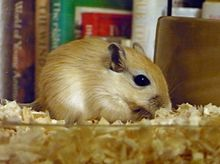
\includegraphics{gerbil}
\end{figure}

\begin{equation}
\alpha + \beta + 1
\end{equation}


Single quotes: `text'.
Double quotes: ``text''.


In March 2006, Congress raised that ceiling an additional \$0.79
trillion to \$8.97 trillion, which is approximately 68\% of GDP. As of
October 4, 2008, the ``Emergency Economic Stabilization Act of
2008'' raised the current debt ceiling to \$11.3 trillion.

% not so good:
Let a and b be distinct positive
integers, and let c = a - b + 1.
% much better:
Let $a$ and $b$ be distinct positive
integers, and let $c = a - b + 1$.

Let $y=mx+b$ be \ldots
Let $y = m x + b$ be \ldots


$y = c_2 x^2 + c_1 x + c_0$


$F_n = F_{n-1} + F_{n-2}$

$\mu = A e^{Q/RT}$



$\Omega = \sum_{k=1}^{n} \omega_k$


The roots of a quadratic equation
are given by
\begin{equation}
x = \frac{-b \pm \sqrt{b^2 - 4ac}}
{2a}
\end{equation}
where $a$, $b$ and $c$ are \ldots


We can write
$ \Omega = \sum_{k=1}^{n} \omega_k $
in text, or we can write
\begin{equation}
\Omega = \sum_{k=1}^{n} \omega_k
\end{equation}
to display it.

\begin{itemize}
% for bullet points
\item Biscuits
\item Tea
\end{itemize}
\begin{enumerate}
% for numbers
\item Biscuits
\item Tea
\end{enumerate}



\end{document}
